\newpage
\hypertarget{emptyPartition tex}{}
\subsection{Implementing empty}
\texHeader

\begin{itemize}
 
\item[$\blacktriangleright$] To initialize your new control flow, you can once again take advantage of eMoflon's auto completion. Inside the
\texttt{empty} declaration, press  \texttt{Ctrl + spacebar} and select \texttt{forEach} from the menu (Fig.~\ref{eclipse:typeCompletion}).

\vspace{1cm}

\begin{figure}[htpb]
\begin{center}
  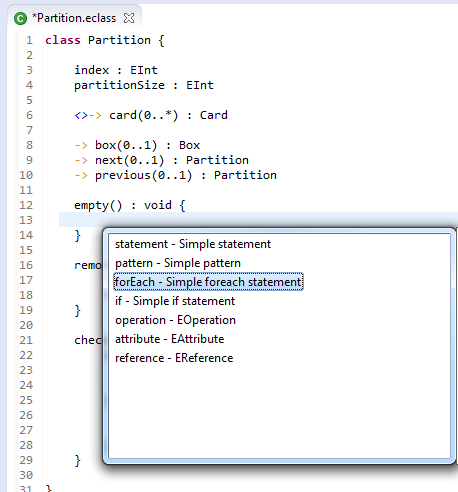
\includegraphics[width=0.7\textwidth]{eclipse_emptyTypeCompletion}
  \caption{eMoflon's auto completion}
  \label{eclipse:typeCompletion}
\end{center}
\end{figure}

\vspace{1cm}

\item[$\blacktriangleright$] Create a single pattern, \texttt{deleteCardsInPartition}. Remove the suggested second pattern as you only need to complete the
deletion -- no extra steps are required in this simple case!

\item[$\blacktriangleright$] Your activity should now resemble Fig.~\ref{eclipse:emptyControlFlow}.

\clearpage

\begin{figure}[htpb]
\begin{center}
  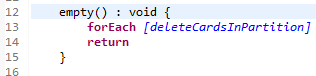
\includegraphics[width=0.5\textwidth]{eclipse_emptyControlFlow}
  \caption{Control flow for \texttt{partition.empty()}}
  \label{eclipse:emptyControlFlow}
\end{center}
\end{figure}

\item[$\blacktriangleright$] While similar to \texttt{removeCard} (Fig.~\ref{eclipse:deleteReference}), this new pattern will go one step further by requesting
a full destruction of \texttt{card}, instead of just deleting the link between the object variables. This means that in addition to destroying the link between
the partition and \texttt{card}, we need to destroy the object variable \texttt{card} as well.

\item[$\blacktriangleright$] Create a \texttt{@this} object variable, and delete its link to \texttt{card} via \syntax{-- -> card:card} Then create another
object variable \texttt{card}, deleting it by prefixing its name with the same \texttt{`--'} operator.

\vspace{0.5cm}

\item[$\blacktriangleright$] Your pattern should now resemble Fig.~\ref{eclipse:emptyPattern}.

\vspace{0.5cm}

\begin{figure}[htpb]
\begin{center}
  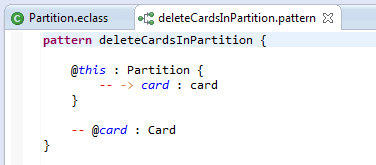
\includegraphics[width=0.6\textwidth]{eclipse_emptyPattern}
  \caption{Destroying both \texttt{card} and the link variable}
  \label{eclipse:emptyPattern}
\end{center}
\end{figure}

\vspace{0.5cm}

\item[$\blacktriangleright$] That's it! Look at you go\ldots you're just speeding through these SDMs now! To see how \texttt{empty} is specified in the visual
syntax, review Fig.~\ref{ea:sdm_end} from the previous section.

\vspace{0.5cm}

\item[$\blacktriangleright$] Although the Learning Box GUI does not have an explicit action that invokes this SDM, feel free to extend it and see your SDM in
action!

\end{itemize}
